\documentclass{article}
\usepackage{hyperref}
\usepackage{fancyhdr}
\usepackage{graphicx}
\usepackage{amsmath}
\usepackage{amssymb}
\usepackage{float}
\usepackage{enumitem}
\usepackage{mathtools}

% if you want to create a new list from scratch
\newlist{alphalist}{enumerate}{1}
% in that case, at least label must be specified using \setlist
\setlist[alphalist,1]{label=\textbf{\alph*.}}

% \graphicspath{{images/}}
\pagestyle{fancy}
\title{EE 271: Final Project Inference Engine on FPGA}
\author{Jay Pankaj Patel}
\date{\today}

\begin{document}
\maketitle
\tableofcontents
\newpage
\section{Building Blocks}
For our inference implementation, I am considering using Convolutional Neural Networks (CNNs). They are an algorithm used to recognize patterns in data. I believe the target data should be handwritten digits from 0--9. Neural networks are built using a collection of neurons organized into layers, each with their own weights and biases. The building blocks of CNNs are the following:
\begin{itemize}
  \item \textbf{Tensor} -- can be thought of as an $n$-dimensional matrix. We need to decide how big to make our tensor. I was considering making it smaller, like three dimensions, because our goal is to perform simple classification.
  \item \textbf{Neuron} -- is a mathematical function that takes multiple inputs and gives a single output.
  \item \textbf{Layer} -- is simply defined as a collection of neurons.
  \item \textbf{Kernel Weights and Biases} -- unique to each neuron and are determined during the training phase of our network. We will train the model on a computer and extract the weights and biases to the FPGA for inference.
  \item \textbf{Differentiable Score Function} -- represented as class scores on the output layer.
\end{itemize}
These are the high-level components needed; let's go over what they mean and the equations associated with them.

\section{Convolutional Module Design: Neuron}
Let's define some terms before we start:

\subsection{Background}
\begin{itemize}
  \item \textbf{What is a feature?} \\
    A feature is an individual measurable property that a model uses to make a prediction or classification.
  \item \textbf{What is a feature map?} \\
    A feature map is the output of all the prevalent features extracted using a filter. In this field, the 'filter' is referred to as a \emph{kernel}. Hence, I will be using "kernel" from this point forward.
  \item \textbf{What is convolution?} \\
    Convolution, in a mathematical sense, is an operation performed on two functions that produces a third function. The mathematical operation is defined as the integral of the two functions after one of them is reflected about the y-axis and shifted. Mathematically:
\end{itemize}

\subsection{Equations}
\begin{align*}
  \left( f  * g \right) \left( t \right) &= \int_{-\infty}^{\infty} f \left( \tau \right) g \left( t - \tau \right) \, d\tau
\end{align*}

Graphically:
\begin{figure}[H]
  \begin{center}
    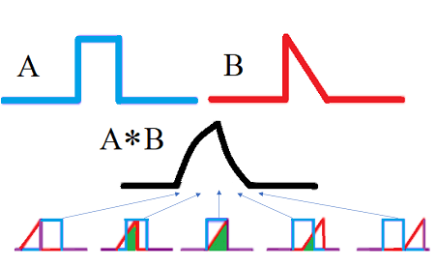
\includegraphics[width=0.5\textwidth]{figures/math_con}
  \end{center}
  \caption{Convolution of two functions A (red) and B (blue) producing a third function describing the overlap (green)}\label{fig:}
\end{figure}

However, this is true for continuous cases. In our case, we are dealing with discrete systems, so the convolution of discrete systems is defined differently. The core definition remains the same; however, the mathematical operation is a summation instead of an integral, as shown:
\begin{align*}
  \left( f * g \right) \left[ n \right] &= \sum_{m = -\infty}^{\infty} f \left[ m\right] g \left[ n-m \right]
\end{align*}

In practicality, since our system has a finite response, there exists a support. A support is defined as a range where our function is nonzero. Hence, the following equation can be rewritten as:
\begin{align*}
  \Aboxed{\left( f * g \right) \left[ n \right] &=  \sum_{m = -M }^{M} f \left[ n - m  \right]  g \left[ m \right]}
\end{align*}

where $g$ has a finite support in the set $ \left\{ -M, -M  + 1,  \dots, M-1, M \right\} $.

In CNNs, the most computationally expensive operation is the convolution layer. It is used to extract image features. The convolution of the input feature map with the weight kernel results in a feature map of this layer after processing by the activation function \cite{xiao_fpga_2020}. The equation is given by:

\begin{align*}
  \Aboxed{  y'_j = f \left( \sum_{i \in M_j}^{} x^{l-1}_{i}  * k^l_{ij} + b^l_{j}\right)}
\end{align*}

\begin{itemize}
  \item $ y^{l}_j $ : Feature map of the $ j $th convolution kernel result of the $ l  $th layer.
  \item $ M_{j} $ : Represents the selection of the previous input feature map by the current convolution.
  \item $ x_{i }^{l-1} $: Represents the previous input feature map.
  \item $ k_{ij}^l  $: Represents the $ i  $th weighting coefficient of the $ j  $th convolution of the $ l  $th layer.
  \item $ b^{l }_j $ : Represents the bias parameter of the $ j  $th convolution kernel of the $ l  $th layer.
  \item $ f $ : The nonlinear activation function.
\end{itemize}

This formula defines a neuron in neural networks, specifically a convolution-based neuron used in CNNs. The weighting coefficients and biases come from the output of a trained model. We will use a pretrained model's weights and biases in our convolution calculations. The weights and biases are given in floating point representation and must be converted to fixed-point. The activation function will most likely be ReLU; however, it may change in the future. Looking at the required computation for each neuron, we can see that this is essentially a multiply-accumulate (MAC) operation. Using this knowledge, we can design a circuit to compute the convolution of each layer efficiently in hardware.



\end{document}
